\documentclass[11pt]{article}
\usepackage[]{authblk}
\usepackage{graphicx}
\usepackage{color}
\usepackage{longtable}
\usepackage{hanging}
\usepackage{indentfirst}
\usepackage{setspace}
\usepackage{verbatim}
\usepackage{upgreek}
\usepackage{framed}
\usepackage{ textcomp }
\usepackage[weather]{ifsym}
\usepackage{natbib}
\usepackage{url}
\usepackage{soul}
\usepackage{amsmath, amsfonts,amssymb,mathrsfs}
\usepackage{fancyhdr}
\usepackage[compact]{titlesec}
\usepackage[T1]{fontenc}
\usepackage{lmodern}

\setlength{\evensidemargin}{0in}
\setlength{\headheight}{0in}
\setlength{\headsep}{0in}
\setlength{\oddsidemargin}{-0.25in}
\setlength{\paperheight}{11in}
\setlength{\paperwidth}{8.5in}
\setlength{\tabcolsep}{0in}
\setlength{\textheight}{9in}
\setlength{\textwidth}{7in}
\setlength{\topmargin}{0in}
\setlength{\topskip}{0in}
\setlength{\voffset}{0in}
%\setstretch{2}
%\raggedright
\parskip = 0.15in
\pagestyle{plain}
\setlength{\parindent}{0cm}

\definecolor{citescol}{RGB}{194,101,1}
%\definecolor{citescol}{RGB}{73,0,165}
\definecolor{urlscol}{RGB}{0,150,206}
%\definecolor{urlscol}{RGB}{0,107,124}
%\definecolor{linkscol}{RGB}{187,24,0}
\definecolor{linkscol}{RGB}{149,0,207}
%\definecolor{linkscol}{RGB}{73,0,165}
\definecolor{mycol}{RGB}{25,23,191}
\definecolor{outputcol}{RGB}{34,139,34}
\definecolor{tcol}{RGB}{165,0,14}


%\def\Fld@bordercolor{1 0 0}
%\renewcommand*{\DefaultHeightofTextMultiline}{6\baselineskip} 
%\renewcommand*{\LayoutTextField}[2]{\makebox[6em][l]{#1 }%
%  \raisebox{\baselineskip}{\raisebox{-\height}{#2}}}
%\def\LayoutChoiceField#1#2{\makebox[6em][l]{#1 }#2}

%\LayoutTextField{label}{field}

\DeclareMathAlphabet{\msfsl}{T1}{cmr}{m}{it}
\DeclareMathAlphabet{\msyf}{OMX}{pcr}{m}{it}
\newcommand{\alf}{\upalpha}
\newcommand{\hilight}[1]{\colorbox{yellow}{#1}}

\newcommand{\levelone}[1]{
\bigskip
\noindent{\LARGE{\textsc{#1}}}
\vspace {0.05in}
}

\newcommand{\leveltwo}[1]{
\bigskip
\noindent{\Large{\textit{#1}}}
\vspace {-1mm}
}

\newcommand{\descriptionhead}[1]{
\noindent{\textbf{\textit{#1}}}\\ \vspace{-7mm}
}

\newcommand{\dhead}[1]{
\noindent{\textbf{\textit{#1 --}}}
}


\newcommand{\exs}[1]{
\vspace{-4mm}
\begin{itemize}
\item #1 \\ \vspace{-8mm}
\end{itemize}
}

\newcommand{\nbo}[1]{{\color{red}{#1}}}


\newcommand{\stepbullet}{\noindent \textbullet \ }
\newcommand{\mi}[1]{\textbf{\textit{#1}}}


\newcommand{\levelthree}[1]{\textit{#1 --}}

%\newcommand{\bowtiecirclefig}{{\rlap{\rlap{{\textbf{\BigCircle}}}{\FilledTriangleLeft}}\FilledTriangleRight}}

\bibliographystyle{bib_tex/mbe}
\bibpunct[; ]{(}{)}{;}{a}{,}{;}


\usepackage[breaklinks]{hyperref}
\usepackage[all]{hypcap}
\hypersetup{colorlinks=true,linkcolor=linkscol,citecolor=citescol,urlcolor=urlscol}


\newcommand{\R}{\texttt{R} }
\newcommand{\TESS}{\texttt{TESS}}
\newcommand{\PBD}{\texttt{PBD}}
\newcommand{\DDD}{\texttt{DDD}}
\newcommand{\Laser}{\texttt{laser}}
\newcommand{\TreePar}{\texttt{TreePar}}
\newcommand{\diversitree}{\texttt{diversitree}}
\newcommand{\RevBayes}{\texttt{RevBayes}}
\newcommand{\Rev}{\texttt{Rev}}
\newcommand{\MrBayes}{\texttt{MrBayes}}
\newcommand{\BEAST}{\texttt{BEAST}}
\newcommand{\PhyloBayes}{\texttt{PhyloBayes}}
\newcommand{\PAML}{\texttt{PAML}}


\usepackage{framed}
\usepackage[]{listings}
\usepackage{fontspec}
\usepackage{placeins}
\usepackage{epstopdf}
\usepackage{hyperref}
\usepackage{enumerate}
\usepackage[font=small]{caption}
\usepackage{float}
\usepackage[table]{xcolor}

\lstset{breaklines=true}

\definecolor{shadecolor}{RGB}{183,207,237}

\setlength{\topmargin}{-0.4in}
\setlength{\headheight}{14.5pt}
%\pagestyle{fancy}

\newcommand{\brm}[1]{{\textcolor{blue}{[BRM comment: #1]}}} % BRM comment

\titlespacing{\section}{0pt}{*0}{*0}
\titlespacing{\subsection}{0pt}{*0}{*0}
\titlespacing{\subsubsection}{0pt}{*0}{*0}

\titleformat{\section}
  {\normalfont\Large\bfseries\color{mycol}}
  {\thesection}{1em}{}

\titleformat{\subsection}
  {\normalfont\large\bfseries\color{mycol}}
  {\thesubsection}{1em}{}

\titleformat{\subsubsection}
  {\normalfont\bfseries\color{mycol}}
  {\thesubsection}{1em}{}

% command for MrBayes command-line step
\newcommand{\cl}[1]{{\texttt{\textbf{#1}}}}
\newcommand{\colx}[1]{{\textcolor{tcol}{#1}}}

\newcommand{\mbcl}[1]{\exs{\cl{MrBayes > {#1}}}}

\newcommand{\rbprmt}{RevBayes > } 
\newcommand{\rbcl}[1]{\exs{\cl{\rbprmt{#1}}}}
\newcommand{\rbout}[1]{\exs{\cl{\textcolor{outputcol}{#1}}}}
\newcommand{\rbdn}{{\Large \symbol{126}}} % This makes a copy/pasteable tilde
\newcommand{\rbclml}[1]{\exs{\cl{\ \ \ \ \ \ \ \ \ \ \ {#1}}}}

% text box settings
% requires compiling w/ XeLaTeX
\newfontfamily\listingsfont[Scale=1.0]{Courier New}
\lstset{basicstyle=\listingsfont, columns=texcl}
\defaultfontfeatures{Mapping=tex-text}

\makeatletter
\lst@CCPutMacro\lst@ProcessOther {"2D}{\lst@ttfamily{-{}}{-{}}}
\@empty\z@\@empty
\makeatother

\renewcommand\bibsection{\subsubsection*{\center \sc References}}

\begin{document}
\begin{titlepage}

\begin{center}
\vfill

\begin{figure}[h] 
\centering 

\includegraphics[height=120mm]{./figures/AutoParts_Logo.png} 
\label{logo}
\end{figure} 

{\huge\bf Automating Bayesian Analysis of\\Partitioned Sequence Datasets}

{\Large \sc Brian R. Moore$^{\,1}$ and John P. Huelsenbeck$^{\,2}$} \\

\medskip

{\em
$\mbox{}^1$Department of Evolution and Ecology, University of California, Davis\\
\vspace{0.4\baselineskip}
Storer Hall, One Shields Avenue, Davis, CA 95616, \mbox{U.S.A.} \\

\smallskip

$\mbox{}^2$Department of Integrative Biology, University of California, Berkeley\\
\vspace{0.4\baselineskip}
3140 VLSB, Berkeley, CA 94720-3140, \mbox{U.S.A.}
}
\vfill
\end{center}




\vfill
\end{titlepage}

\newpage
\section*{Background}
\noindent
Our motivation for developing \verb!AutoParts! is to estimate phylogeny under a model that accommodates process heterogeneity---variation in the evolutionary process across the sequence alignment---within a flexible Bayesian statistical framework. 

We define a \emph{partition scheme} as the number of distinct substitution processes and the assignment of (subsets of) nucleotides sites to those distinct processes.
Our solution for accommodating process heterogeneity treats the partition scheme as a random variable described by the Dirichlet process prior (DPP) model.
Numerical integration (MCMC simulation) is then used to estimate parameters of the phylogenetic model---the tree topology, branch lengths and substitution model parameters---while averaging over all possible partition schemes.

The user is required to specify the sequence alignment, the data partitions (the subsets of nucleotide sites intended to capture process heterogeneity), and the hyper parameters of the DPP model. 
Parameters of the DPP model include (1) the `concentration' parameter, $\alpha$, which controls the expected number of partition schemes, and (2) the `base measure', $G_0$, which specifies the prior probability density for each substitution model parameter. 

\verb!AutoParts! implements a Dirichlet process for each of the four substitution model parameters: the stationary frequencies, the exchangeability rates, the tree length, and the alpha parameter controlling the degree of among-site rate variation. 
The Dirichlet processes for the four substitution model parameters share a common concentration parameter, which can be specified either as a fixed value or treated as a random variable (described by a second-order gamma hyperprior).

In this guide, we briefly describe how to install \verb!AutoParts!, and then walk through a simple analysis of the included conifer dataset, illustrating how to generate and interpret results.

Details of the methods implemented in \verb!AutoParts! are described in the following paper: \\ \vspace{-7mm}

\hangindent=1cm Moore, B. R., J. McGuire, F. Ronquist, and J. P. Huelsenbeck. (in review) Bayesian analysis of partitioned\\
data. \emph{Systematic Biology}.

Details of the \verb!AutoParts! software are described in the following paper: \\ \vspace{-7mm}

\hangindent=1cm Moore, B. R., S. H\"{o}hna, and J. P. Huelsenbeck. (in review) Automating the Bayesian analysis of partitioned\\
sequence datasets with AutoParts. \emph{Bioinformatics}.

\bigskip
\section*{Installing AutoParts}

Download the \verb!AutoParts! archive, decompress it, and move it to the desired location on your computer.
If you are using a Mac OS, you may be able to use the pre-compiled binary included with the \verb!AutoParts! distribution.
To execute the binary, navigate to the \cl{bin} directory within the \verb!AutoParts! bundle:

\cl{cd users/<path to AutoParts directory on your computer>AutoParts/bin/ <return>}

Next, execute the program by typing:
\cl{./AutoParts <return>}

If the precompiled binary is not compatible with your OS, you can compile it from the included source code using the \verb!cmake! utility.
Point your terminal to the directory that contains the \verb!AutoParts! source code, which is located in the program bundle:

\cl{cd users/<path to AutoParts directory on your computer>AutoParts/src/ <return>}

Next, compile the program by first typing:

\cl{cmake . <return>}

followed by:

\cl{make <return>}

If you do no have \verb!cmake! installed, you can install it using the \verb!homebrew! package-manager utility by typing:

\cl{brew install cmake <return>}
  
If you do no have the \verb!homebrew! package-manager utility, you can install it by first navigating to your home directory by typing:

\cl{cd <return>}

and then typing the following in your terminal window:

\cl{ruby -e "\$(curl -fsSL https://raw.github.com/Homebrew/homebrew/go/install)" <return>}


If you want to be able to execute \verb!AutoParts! from any directory on your computer, you can add it to your path environment variable.
On a Mac, this can be achieved by editing the \verb!.bash_profile! file.
On my laptop, the \verb!AutoParts! binary is located in the path \cl{usr/Applications/AutoParts/src/}; I will add this path to my bash profile using the \verb!vi! text editor.
Type:

\cl{vi .bash\_profile <return>}

The \verb!vi! editor will display something like this: \\ \vspace{-15mm}

\begin{center}
\end{center}
{\tt \scriptsize \begin{framed}
\begin{lstlisting}
# Setting PATH for Python 2.7
# The orginal version is saved in .bash_profile.pysave
PATH="/Library/Frameworks/Python.framework/Versions/2.7/bin:${PATH}"
export PATH
export PATH="/usr/Applications/mrbayes_3.2.2/src/:$PATH"
export PATH="/usr/Applications/RevBayes/src/:$PATH"
~                                                                                                                           
~                                                                                                                           
~                                                                                                                           
".bash_profile" 8L, 423C
\end{lstlisting}
\end{framed}}

  
Type \cl{i} to switch to \cl{INSERT} mode, enter the path to the \verb!AutoParts! binary, press the \cl{<Esc>} key to go back to \cl{command} mode, and then type \cl{:wq} to save and quit. 
Finally, type \cl{source ~/.bash\_profile <return>} to reload the Terminal so it will read in the new path.

Now you can execute \verb!AutoParts! from any directory on your computer by typing \cl{AutoParts <return>}.


\bigskip
\section*{Input file format}

\verb!AutoParts! uses a simple \verb!Phylip!-style input file format.
This is a plain text file that includes three main pieces of information:
\begin{enumerate}
\item{The number of species followed by the number of sites (specified in first line of the file)} \\ \vspace{-7mm}
\item{The multiple sequence alignment} \\ \vspace{-7mm}
\item{The set of two or more predefined data partitions (specified as charsets at the end of the file)}
\end{enumerate}

For example, here is part of the input file for the included example file, \cl{conifer.in}  (showing the first 12 sites of the sequence alignment):
\begin{center}
{\bf Box 1:} A fragment of the input file containing the $9$ conifer species in the included example dataset. \\
\end{center}
{\tt \scriptsize \begin{framed}
\begin{lstlisting}
9 2659
Ginkgo_biloba             TTATTGGTCCAG...
Araucaria_araucana        -----GGTCCGG...
Cedrus_deodara            TCATTGGCCCAG...
Cupressus_arizonica	  ------------...
Juniperus_communis        ------------...
Pinus_densiflora          TCATTGGCCCAG...
Podocarpus_chinensis      TCATCGGCCCTG...
Sciadopitys_verticillata  TCATTGGTCCAG...
Taxus_baccata             TTATCGGCCCAG...
charset atpB_1st = 1-1394\3;
charset atpB_2nd = 2-1394\3;
charset atpB_3rd = 3-1394\3;
charset rbcL_1st = 1395-2659\3;
charset rbcL_2nd = 1396-2659\3;
charset rbcL_3rd = 1397-2659\3;
\end{lstlisting}
\end{framed}}

\bigskip
Our example file contains an alignment for $9$ conifer species with $2659$ sites sampled from two chloroplast protein-coding genes, atp\emph{B} and rbc\emph{L}.
It is up to the user to specify a set of data partitions that are likely to capture patterns of process heterogeneity across the alignment.
In this case, for example, we might specify two data partitions, one for the atp\emph{B} gene and the second for the rbc\emph{L} gene.
Alternatively, we might specify three data partitions corresponding to the three codon positions of both protein-coding genes.
In any case, the set of data partitions that we specify becomes a \emph{fixed assumption of the analysis}.

Note, however, that it is possible to explore alternative data-partitioning schemes---performing a separate analysis under each candidate scheme---and then choosing among them based on the marginal likelihoods of competing schemes.   
Generally, we recommend erring on the side of defining more granular data partitions: if the evolutionary process is uniform within two pre-specified data partitions, they will be grouped together under the DPP model.
Here, we have decided to define separate partitions for the three codon positions in each of the two genes, for a total of $K = 6$ data partitions.

\newpage
\section*{Specifying details of the analysis}

In this guide, we will use \verb!AutoParts! interactively by typing commands in the command-line console.
%We use \colorbox{shadecolor}{\tt blue shaded boxes} to delineate \verb!AutoParts! commands that you should type (or copy/paste) at \verb!AutoParts! prompt. 
To see a list of available commands, you can execute \verb!AutoParts! and view the splash page:

\begin{center}
{\bf Box 2:} The \verb!AutoParts! splash page listing available commands. \\
\end{center}
{\tt \scriptsize \begin{framed}
\begin{lstlisting}
Usage:
   -i : Input file name
   -t : Tree file name (for constraining the analysis to a fixed tree)
   -o : Output file name
   -l : Number of MCMC cycles
   -d : Number of MCMC cycles to discard as the "burn-in"
   -p : Print frequency
   -s : Sample frequency
   -b : Exponential parameter for branch lengths
   -g : Number of discrete gamma rate categories
   -e : Exponential parameter for shape parameter describing ASRV
   -c : Concentration parameter is fixed (1) or a random variable (0)
   -k : Prior mean of the number of categories when the concentration parameter is fixed
   -m : Prior mean of the concentration parameter when it is a random variable
   -v : Prior variance of the concentration parameter when it is a random variable
  -t1 : MCMC tuning parameter for the tree topology parameter
  -t2 : MCMC tuning parameter for the gamma shape parameter
  -t3 : MCMC tuning parameter for the base frequencies
  -t4 : MCMC tuning parameter for the substitution rates
  -t5 : MCMC tuning parameter for the tree length parameter

Example:
   ./AutoParts -i <input file> -o <output file>
\end{lstlisting}
\end{framed}}

We will specify details for an analysis of the conifer dataset, where we fix the concentration parameter (using the \cl{-c 1} argument) such that the prior mean on the expected number of process patrons, $E(k)$, is centered on an intermediate value for the $K=6$ data partitions (using the \cl{-k 3.0} argument).
We will run the chain for $100,000$ cycles (using the \cl{-l 100000} argument) and thinned by sampling every $100$ cycles (using the \cl{-s 100} argument), and we will have it print to the screen at the same frequency (using the \cl{-p 100} argument).
It will generally be necessary to carefully diagnose the MCMC output to assess whether the chain has converged to the stationary distribution, and if so, to identify the fraction of the pre-stationary samples that should be discarded as burn-in.
For the moment, however, we  will boldly pre-specify the burn-in as the first half of the samples (using the \cl{-d 50000} argument).

The details of this analysis are specified by the following command-line string:

%{\tt \begin{snugshade*}
%\begin{lstlisting}
\cl{AutoParts -i conifer.in -o conifer -l 100000 -p 100 -s 100 -d 50000 -c 1 -k 3.0 <return>}
%\end{lstlisting}
%\end{snugshade*}}

Note that the screen output is automatically written to a file called \cl{<output\_file\_name>.log}, which contains important summary information and diagnostics that we will discuss below.
For this reason, 
%you should avoid redirecting the screen output using the redirect operator, \cl{>}, as it may overwrite the log file.
%Also, 
it's generally a good idea to match the sampling and printing frequencies (using the \cl{-s} and \cl{-p} arguments).


\newpage
\section*{Running the analysis}

Hit \cl{<return>} to start the MCMC simulation (the analysis required $\sim 5$ minutes to complete on my laptop).
When the analysis begins, it reports the state sets---the number of process partitions for each of the four parameters, the assignment of data partitions to those process partitions, and the parameter values for the process partitions:

\begin{center}
{\bf Box 3:} The start of the \verb!AutoParts! screen output. \\
\end{center}
{\tt \scriptsize \begin{framed}
\begin{lstlisting}
   AutoParts v.1.0
   John Huelsenbeck & Brian Moore
   University of California, Bervis

   Setting up state sets
alpha fixed to 1.69577
Table 1
Patrons at table: "012345"
   0 (9, -1, -1) 0.00000 (Ginkgo_biloba)  <- Root
     9 (10, 14, 0) 0.00897
       10 (1, 3, 9) 0.04196
         1 (-1, -1, 10) 0.03625 (Araucaria_araucana) 
         3 (-1, -1, 10) 0.09207 (Cupressus_arizonica) 
       14 (15, 11, 9) 0.25955
         15 (7, 8, 14) 0.02357
           7 (-1, -1, 15) 0.01012 (Sciadopitys_verticillata) 
           8 (-1, -1, 15) 0.00880 (Taxus_baccata) 
         11 (12, 2, 14) 0.04422
           12 (13, 5, 11) 0.00523
             13 (4, 6, 12) 0.03358
               4 (-1, -1, 13) 0.11893 (Juniperus_communis) 
               6 (-1, -1, 13) 0.20797 (Podocarpus_chinensis) 
             5 (-1, -1, 12) 0.00497 (Pinus_densiflora) 
           2 (-1, -1, 11) 0.10382 (Cedrus_deodara) 
alpha fixed to 1.69577
Table 1
Patrons at table: "04"
alpha = 0.19929
Table 2
Patrons at table: "1"
alpha = 0.29665
Table 3
Patrons at table: "235"
alpha = 1.95620
\end{lstlisting}
\end{framed}}

The output first indicates the value (and treatment) of the concentration parameter, which for this analysis is \cl{alpha fixed to 1.69577}: this value centers the prior for the number of process partitions to the specified value, $E(k)=3.0$.
Note that $\alpha$ is conventionally used for the concentration parameter of the DPP model, as it is in \verb!AutoParts!. 
In our paper (Moore et al., in review), however, we used $\chi$ for this parameter.  
Our motivation was to avoid confusion between the concentration parameter of the DPP model and the familiar $\alpha$-shape parameter of the discrete-gamma model used to accommodate among-site rate variation (ASRV).

The output specifies the initial state of the chain with respect to the process partitions for each parameter in the following order: tree topology, alpha-shape parameter, the exchangeability/substitution rates, base frequencies, and tree length.
By assumption, all $K=6$ data partitions share the same process partition for the tree parameter.
The `value' of the tree parameter (the topology) has been drawn from its `base measure'---the uniform prior distribution on tree topologies---and is depicted in tab-delimited format.

Next, the output describes the initial process partition for the alpha-shape parameter.
Three process partitions have been sampled.
Data partitions $0$ and $4$ (corresponding to the first codon positions of atp\emph{B} and rbc\emph{L}, see Box 1) have been assigned to the first process partition, which has an alpha value of $0.19929$.
Data partition $1$ (corresponding to the second codon position of atp\emph{B}) has been assigned to the second process partition with a parameter value of $0.29665$.
Finally, the remaining data partitions, $2, 3, 5$ (corresponding to the three codon positions of rbc\emph{L}, have been assigned to the third process partition with a parameter value of $1.95620$.
Again, this initial partition scheme for the $\alpha$-shape parameter is based on a random draw from the DPP model.
The concentration parameter controls the number of process partitions and the assignment of data partitions to tables.
The base measure, $G_0$, is the prior from which parameter values are drawn (we use an exponential prior for the $\alpha$-shape parameter controlling the degree of ASRV).

The output continues in this way, describing the full model specification that corresponds to the initial (and random) state of the chain. 
Samples are then written to the screen at the specified interval (here every $100$ cycles):

\begin{center}
{\bf Box 3:} The first 15 samples from the MCMC simulation. \\
\end{center}
{\tt \scriptsize \begin{framed}
\begin{lstlisting}
   Gen -- lnL         -- Number of occupied tables    -- Parameter update
   100 -- -9949.634 -- t(1) rv(3) sr(3) bf(2) tl(4) -- updating tree
   200 -- -9767.748 -- t(1) rv(3) sr(2) bf(3) tl(4) -- updating tree
   300 -- -9684.823 -- t(1) rv(3) sr(2) bf(2) tl(3) -- updating subrates
   400 -- -9685.444 -- t(1) rv(3) sr(2) bf(2) tl(3) -- updating tree
   500 -- -9646.255 -- t(1) rv(3) sr(2) bf(2) tl(3) -- updating tree
   600 -- -9629.956 -- t(1) rv(3) sr(2) bf(2) tl(3) -- updating tree
   700 -- -9603.426 -- t(1) rv(3) sr(2) bf(2) tl(4) -- updating tree
   800 -- -9596.978 -- t(1) rv(3) sr(3) bf(2) tl(4) -- updating tree
   900 -- -9600.097 -- t(1) rv(3) sr(2) bf(2) tl(3) -- updating tree
  1000 -- -9613.031 -- t(1) rv(4) sr(3) bf(2) tl(3) -- updating tree
  1100 -- -9547.029 -- t(1) rv(2) sr(3) bf(2) tl(5) -- updating basefreq
  1200 -- -9587.855 -- t(1) rv(2) sr(2) bf(2) tl(4) -- updating subrates
  1300 -- -9529.674 -- t(1) rv(3) sr(3) bf(2) tl(4) -- updating tree
  1400 -- -9482.361 -- t(1) rv(3) sr(2) bf(2) tl(4) -- updating tree
  1500 -- -9462.873 -- t(1) rv(3) sr(3) bf(2) tl(4) -- updating tree
\end{lstlisting}
\end{framed}}

For each sample, the screen logs the generation of the MCMC, the log likelihood ($ln$L), the number of process partitions for each of the five parameters, and the parameter that is currently being operated on.
For example, the tenth sample (generation $1000$), there is one process partition for the tree topology, \cl{t(1)}, the alpha-shape parameter has four process partitions, \cl{rv(4)}, there are three process partitions for the  substitution rates, \cl{sr(3)}, there are two process partitions for the base frequencies, \cl{bf(2)}, and one process partition for the tree length, \cl{tl(1)}.
At that cycle, a change to the tree topology has been proposed.

When the MCMC simulation is complete, several output files will be generated:\\ \vspace{-7mm}
\begin{enumerate}

\item{Sampled partitions for each model parameter: \cl{<input\_file\_name>.<parameter>.part}} \\ \vspace{-7mm}

\item{Sampled values for each model parameter: \cl{<input\_file\_name>.<parameter>.out}} \\ \vspace{-7mm}

\item{A majority-rule consensus of sampled trees: \cl{<input\_file\_name>mrc.tre}} \\ \vspace{-7mm}

\item{A credible set of sampled trees: \cl{<input\_file\_name>CI.trees}} \\ \vspace{-7mm}

\item{Sampled log-likelihood values: \cl{<input\_file\_name>.lnL}} \\ \vspace{-7mm}

\item{A log of the screen output: \cl{<input\_file\_name>.log}} \\ \vspace{-7mm}

\end{enumerate}

\bigskip
\section*{Interpreting the results}

When the MCMC analysis is complete, \verb!AutoParts! automatically computes some useful values that are written to the \cl{.log} file.
Specifically, it reports the acceptance rates to help assess mixing of the MCMC simulation: as a rule of thumb, acceptance rates should fall within the $20\%-70\%$ range.
It also calculates the various estimates of the marginal likelihood, including the AICM \citep[][]{Raftery07}, the original \citep{newton94} and modified \citep[][]{suchard01} harmonic-mean estimator, and the smoothed marginal-likelihood estimator.
In principle, these marginal likelihoods could be used to evaluate various hypotheses using Bayes factors \citep[{\it e.g.},][]{suchard01}.
We caution, however, that these marginal-likelihood estimates are extremely crude and should only be used as a very rough guide.
Rigorous hypothesis tests will require more stable marginal-likelihood estimates, which could be estimated using thermodynamic integration \citep[{\it e.g.},][]{lartillot06} and/or stepping-stone simulation \citep[{\it e.g.},][]{fan11,xie11}.   

\begin{center}
{\bf Box 4:} Some summary statistics computed at the end of the MCMC simulation. \\
\end{center}
{\tt \scriptsize \begin{framed}
\begin{lstlisting}
Acceptance Rates:
Parameter   Tries  Accep     Rate
tree        42787   4985     0.12
asrv        14149  12947     0.92
subrates    14377  10790     0.75
basefreq    14304   8326     0.58
treelength  14383  12144     0.84

Marginal lnL Estimates:
AICM                           = -19273.99
Harmonic mean (old way)        = -9422.36
Harmonic mean (Suchard)        = -9422.36
Marginal likelihood (smoothed) = -9383.81
\end{lstlisting}
\end{framed}}

Next, \verb!AutoParts! summarizes information regarding inferred patterns of process heterogeneity.
This information is reported for each of the model parameters in the following order: the topology (\cl{tree}), alpha-shape parameter the topology (\cl{asrv}), exchangeability parameters (\cl{subrates}), stationary frequencies (\cl{basefreq}), and tree length (\cl{treelength}).

For each parameter, \verb!AutoParts! reports some useful and interesting summaries:
\begin{enumerate}

\item{The mean partition scheme (the `average partition')} \\ \vspace{-7mm}

\item{The marginal and cumulative probability of sampled process partitions} \\ \vspace{-7mm}

\item{The posterior and prior probability for the number of process partitions} \\ \vspace{-7mm}

\item{The probability that any pair of data partitions belong to the same process partition} \\ \vspace{-7mm}

\end{enumerate}

Let's explore these summaries for the $\alpha$-shape parameter, depicted below (Box 5): 

\newpage
\begin{center}
{\bf Box 5:} Summary of the inferred pattern of process heterogeneity for the alpha-shape parameter. \\
\end{center}
{\tt \scriptsize 
\begin{framed}
\begin{lstlisting}[label=lst:box5]
Restaurant: asrv
   Average Partition = (1,2,1,3,3,3) [6,3]
   Unique partitions:
       1 -- 41941 0.8388 0.8388 (1,2,1,3,3,3) [6,3]
       2 --  7536 0.1507 0.9895 (1,2,3,4,4,4) [6,4]
       3 --   362 0.0072 0.9968 (1,2,1,3,4,3) [6,4]
       4 --    82 0.0016 0.9984 (1,2,3,4,5,4) [6,5]
       5 --    42 0.0008 0.9992 (1,2,1,3,4,4) [6,4]
       6 --    35 0.0007 0.9999 (1,2,1,2,2,2) [6,2]
       7 --     3 0.0001 1.0000 (1,2,1,3,2,3) [6,3]
   Posterior and prior probability distributions for the number of tables:
       1 --     0 0.0000 0.0692
       2 --    35 0.0007 0.2560
       3 -- 41944 0.8389 0.3659
       4 --  7940 0.1588 0.2340
       5 --    82 0.0016 0.0670
       6 --     0 0.0000 0.0079
   Probability that patrons are seated at the same table:
      1    2 -- 0.0000
      1    3 -- 0.8476
      1    4 -- 0.0000
      1    5 -- 0.0000
      1    6 -- 0.0000
      2    3 -- 0.0000
      2    4 -- 0.0007
      2    5 -- 0.0008
      2    6 -- 0.0007
      3    4 -- 0.0000
      3    5 -- 0.0000
      3    6 -- 0.0000
      4    5 -- 0.9902
      4    6 -- 0.9992
      5    6 -- 0.9911
\end{lstlisting}
\end{framed}}

\bigskip
\subsection*{1. Process partitions}
First, \verb!AutoParts! reports the mean partition scheme for the $\alpha$-shape parameter: this is the partition scheme that minimizes the squared distance to all other sampled partition schemes for this parameter \citep[][]{gusfield02}.
The mean partition scheme is rendered in `restricted-growth form' (RGF) notation \citep{stanton86}.
Here, the mean partition scheme for the $\alpha$-shape parameter (in RGF notation) is $(1,2,1,3,3,3)$.
This indicates that the six data partitions are distributed among three process partitions as follows: the first and third data partitions (the first and third codon-position sites of the atp\emph{B} gene region) share a common degree of among-site rate variation, the degree of ASRV for the third data partition (the second codon position of the atp\emph{B} gene region) is inferred to be unique, and data partitions 4, 5, and 6 (for the three codon-positions of the  rbc\emph{L} gene region) are inferred to share a common degree of ASRV. 

Indeed, the process partition for the $\alpha$-shape parameter inferred under the DPP model agrees well with the corresponding estimates of the marginal posterior probability densities for these data partitions, plotted below (Figure \ref{alpha}) by loading the corresponding log file (\cl{conifer.asrv.out}) in \verb!Tracer! \citep{rambaut07}.

\newpage

\begin{figure}[H] 
\centering 
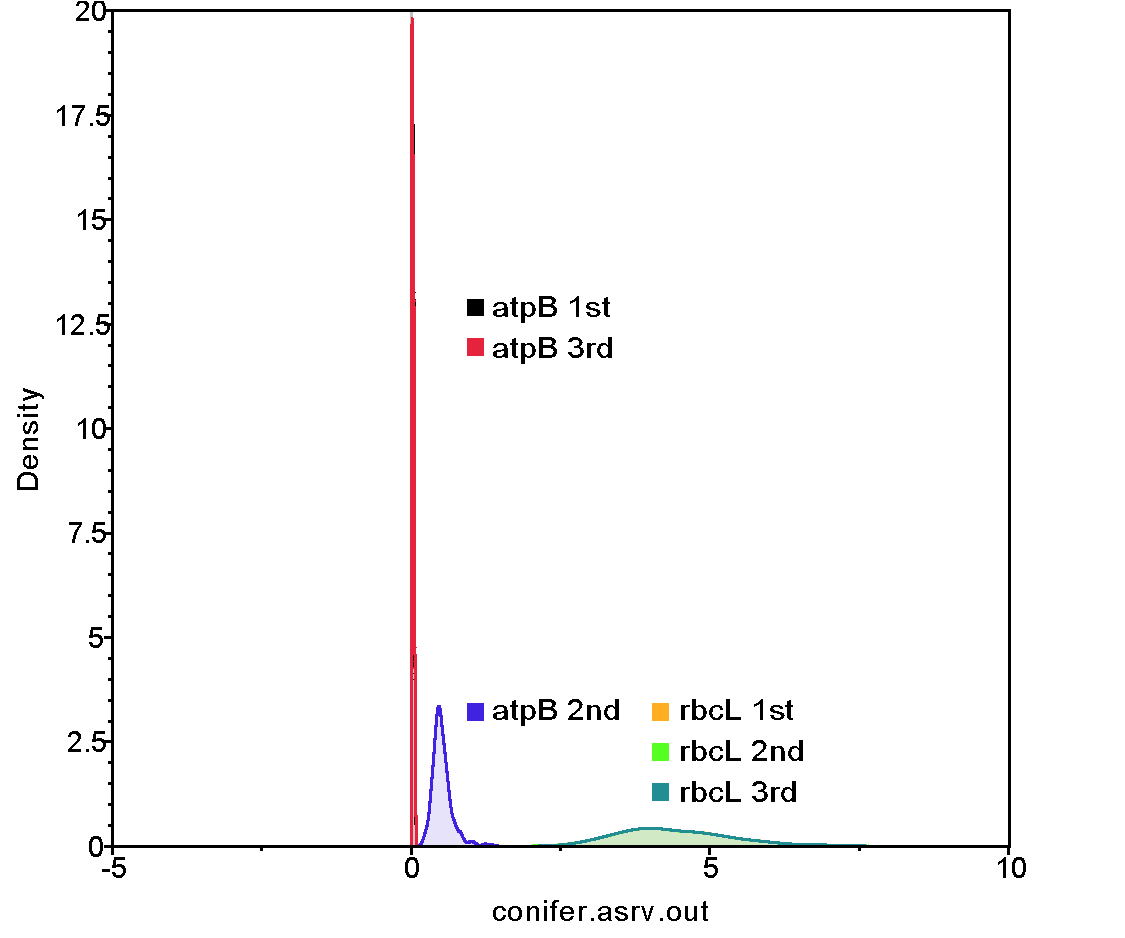
\includegraphics[width=95mm]{./figures/alpha_marginals.pdf} 
\caption{Inferred patterns of among-site substitution rate variation within the conifer sequence alignment.  The marginal posterior probability densities are plotted from the corresponding log file for the $\alpha$-shape parameter (\cl{conifer.asrv.out}) estimated for each of the $K = 6$ predefined data partitions.}
\label{alpha}
\end{figure} \vspace{-5mm}

The process partitions for all four substitution-model parameters are summarized in Figure \ref{partition_scheme}.
We provide an \verb!R! script (\verb!AutoPlots.R!) that will generate this figure from the \cl{conifer.log} file.

\begin{figure}[H] 
\centering 
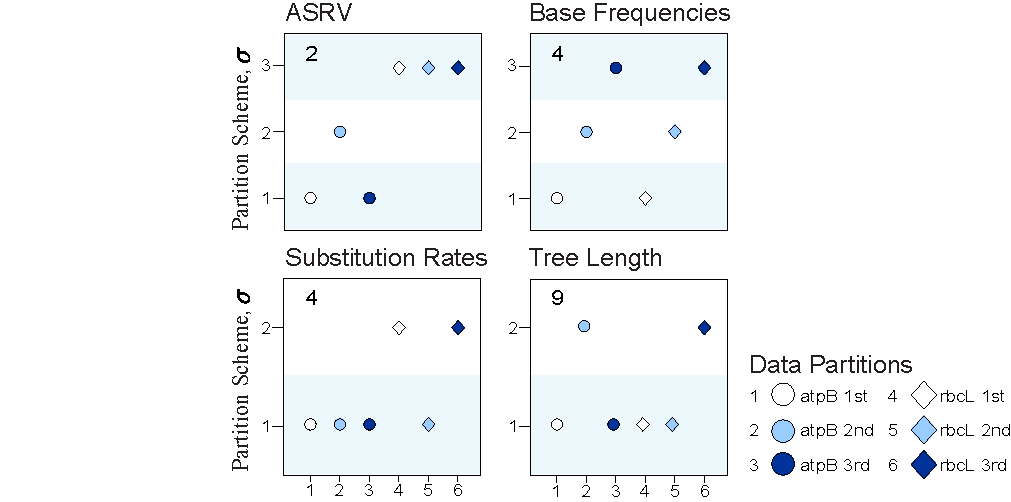
\includegraphics[width=130mm]{./figures/partition_scheme.pdf} 
\caption{Summarizing process heterogeneity in conifers. 
%The partition scheme, $\sigma$, for each of the four parameters specifies both the number of process partitions, $k$, and the allocation vector, ${\mathbf z}$, of the $K = 6$ data partitions to those $k$ process partitions. 
For example, the $K=6$ data partitions are allocated to $k = 3$ distinct process partitions for the $\alpha$-shape parameter (the shaded rows of the panel), where the allocation vector is ${\mathbf z}  = (1,2,1,3,3,3)$ (depicted by the assignment of the data-partition symbols to their respective rows). The number of process partitions in the $95\%$ credible set is depicted in the upper left of each panel.}
\label{partition_scheme}
\end{figure} \vspace{-5mm}

To use \texttt{AutoPlots.R}, navigate to the \cl{AutoPlots} directory within the \verb!AutoParts! bundle: \vspace{-1.5mm}

\cl{cd users/<path to AutoParts directory on your computer>AutoParts/AutoPlots/ <return>}\vspace{-1.5mm}

Now execute \verb!AutoPlots.R! by typing: \cl{Rscript AutoPlots.R --args <path\_to\_file><input\_file\_name>.slog}. \vspace{-6.5mm}

A figure named \cl{<input\_file\_name>.pdf} will be written to the same directory as the \cl{.slog} file. \vspace{-1.5mm}

\bigskip
\subsection*{2. Marginal and cumulative probability of unique process partitions}
The \verb!AutoParts! post-analysis report lists each unique process partition ordered by marginal posterior probability (Box 5). 
This facilitates identification of the $95\%$ credible interval (CI) of process partitions, {\it i.e.}, by adding the marginal probability for the first process partition to that for the second process partition, and then adding this sum to the marginal probability for the third process partition, and so on, until the \emph{cumulative} probability is equal to or greater than $0.95$.
The size of the $95\%$ CI therefore indicates the degree of uncertainty in the estimated process partition for each parameter.
The size of the credible set for each parameter is depicted in the upper-left corner of the corresponding panel in Figure \ref{partition_scheme}. 


\bigskip
\subsection*{3. Posterior and prior probability for the number of process partitions}
The DPP model allows us to calculate the prior probability for the number of process partitions, $k$, given a specified value for the concentration parameter, $\alpha$ and the number of data partitions, $K$:
\begin{align} \label{eq:P(k)}
\mathbb{P}(k \mid \alpha, K) = \frac{{\cal S}_1(K,k) \alpha^k}{\prod\limits^{K}_{i=1}(\alpha + i - 1)},
\end{align}
where ${\cal S}_1(\cdot,\cdot)$ is the Stirling number of the first kind, which specifies the possible permutations of $K$ data partitions among $k$ process partitions:
$$
\mathcal{S}_1(n, k) = (-1)^{n-k} {n \choose k}.
$$

\verb!AutoParts! reports the prior probabilities (computed analytically using the above equations) and the corresponding posterior probabilities (estimated numerically using MCMC) for the number of process partitions for each of the substitution model parameters.
For example, the post-analysis summary reports the prior/posterior probabilities ($P = 0.3659, 0.8389$, respectively) of $k = 3$ process partitions for the $\alpha$-shape parameter (Box 5). 
This provides an efficient and flexible framework for comparing competing models/testing alternative hypotheses regarding the nature of process heterogeneity in molecular evolution (discussed below).

\bigskip
\subsection*{4. Posterior probability that two data partitions share the same process partition}

The DPP model also allows us to calculate the prior probability that any two data partitions, $x_i, x_j$ belong to the same process partition, given a specified value for the concentration parameter, $\alpha$:
\begin{align} \label{eq:P(x_i=x_j)}
\mathbb{P}(x_i = x_j \mid \alpha) = \frac{1}{1+\alpha}.
\end{align}

As in the case for the number of process partitions, the prior probabilities that two data parts share the same process partition (which can be calculated analytically using the above equation) can be compared to the corresponding posterior probabilities (which are estimated numerically using MCMC). 
For example, the post-analysis report indicates that data partitions $1$ and $3$ (the first and third position sites of the atp\emph{B} gene) share the same process partition for the $\alpha$-shape parameter with probability $P = 0.8476$ (Box5).


\bigskip
\section*{Diagnosing MCMC performace and assessing prior sensitivity} \vspace{-1.1mm}

\emph{Diagnosing MCMC performance.}---Model-based inference is, after all, based on the model. 
Careful research means being vigilant regarding the choice of model and also rigorously assessing our ability to estimate under the chosen model. 
The first issue---model specification---is critically important for the simple reason that unbiased estimates can only be obtained under a model that provides a reasonable description of the process that gave rise to our data. 
The DPP model implemented in \verb!AutoParts!  is particularly attractive because it effectively obviates need to select among (mixed) models by virtue of averaging inference of phylogeny over all possible process partitions. \vspace{-1.7mm}

The second issue---rigorously assessing the ability to obtain reliable estimates under the chosen model(s)--- typically receives less attention. 
The implicit assumption, it seems, is that if a model is implemented correctly, and if that implementation is used to obtain an estimate from a given dataset, then we must have performed valid inference under the model. 
This would be perfectly sound reasoning if inferences were based on analytical methods. 
Owing to the complexity of the models, however, it is not possible to estimate phylogenetic model parameters analytically. 
Instead, parameter estimates are based on numerical methods. 
In the Bayesian statistical framework, we use Markov chain Monte Carlo (MCMC) algorithms to approximate the joint posterior probability density of phylogenetic parameters. 
We may be comforted to know that, in theory, an \emph{appropriately constructed} and \emph{adequately run} MCMC simulation is guaranteed to provide an arbitrarily precise description of the posterior probability density \citep[][]{tierney94}.
In practice, however, even a given MCMC algorithm that provides reliable estimates in \emph{most} cases will nevertheless fail in \emph{some} cases and is not guaranteed to work for any particular dataset. 
This raises an obvious question: “When do we know that an MCMC algorithm provides reliable estimates for a given empirical analyses”. 
The answer is simple: \emph{Never}. \vspace{-1.7mm}

Accordingly, the general dictum of Bayesian inference---vigilant diagnosis of MCMC performance---is particularly crucial for estimation of phylogeny (and other model parameters) under high-dimensional mixture models, such as the Dirichlet process prior approach implemented in \verb!AutoParts!. 
We recommend carefully evaluating the output generated by \verb!AutoParts! using diagnostic tools such as \verb!bonsai! (May et. al. 2014). 
Poor mixing for a given parameter can be addressed by altering the value of the corresponding tuning parameter (Box 2). 
The tuning parameters control the magnitude of the proposed changes to current parameter values. 
If acceptance rates for a parameter are too low, the value of the corresponding tuning parameter should be decreased (and vice versa); this is achieved using the \cl{-t<integer>} arguments (Box 2). 
Some aspects of the MCMC output under the DPP model warrant brief comment. 
For example, although multi-modal marginal posterior probability densities are generally cause for concern, under the DPP they may be innocuous. 
Because of the discrete nature of process partitions, the marginal posterior probability density for a parameter may exhibit more than one mode if there is uncertainty regarding the allocation of that data partition to alternative (discrete) process partitions. \vspace{-1.7mm}

In fact, the identification of a multi-modal marginal posterior probability densities may indicate that the pre-defined data partition includes residual process heterogeneity for that parameter. 
Imagine, for example, that we defined a data partition comprising all of the second-position sites of the atp\emph{B} gene, and---after running the analysis---observed that the marginal posterior probability density for this data partition had two modes for the tree-length parameter: one at a lower substitution rate, and the other at a higher rate. 
This might be evidence of a pathological parameter interaction ({\it e.g.}, between the $\alpha$-shape and tree-length parameters). 
On the other hand, the multiple modes may indicate that the data partition as specified contains residual variation in overall substitution rate; for example, some subset of these second position sites may be under positive selection. 
Careful MCMC diagnosis is required to validate the approximation of the joint posterior probability density, and may also provide opportunities to make novel insights into the processes that gave rise to your data. \vspace{-1.7mm}

\bigskip
\emph{Exploring the impact of the concentration parameter.}---The Bayesian statistical framework views parameters as random variables, which requires that we specify probability distributions describing the nature of their random variation. 
Formally, a prior specifies our belief about the parameter values \emph{before} evaluating the data at hand. 
The chosen prior is then updated by the information in the data via the likelihood function, transforming it into the corresponding posterior probability distribution (reflecting our beliefs about the parameter value \emph{after} evaluating the data at hand). 
Because the posterior probability is proportional to the product of the likelihood and the prior, the chosen prior will always influence the posterior to \emph{some} degree. 
This naturally raises concerns regarding the sensitivity of our estimates to the chosen prior.
The DPP model implemented in \verb!AutoParts! has two main priors: the concentration parameter, $\alpha$---which controls the expected number of process partitions, $E(k)$ and the allocation of data partitions among those process partitions, ${\mathbf z}$---and the base measure, $G_0$, which controls the prior values for each process partition.
The base measures implemented in \verb!AutoParts! are the generally familiar prior probability distributions for phylogenetic model parameters: \vspace{-5mm}

\begin{eqnarray*}
\tau & \sim & \mbox{Discrete Uniform}(1, \ldots, B(S)) \\
{\mathbf p} & \sim & \mbox{Dirichlet}(1, 1, \ldots, 1) \\
T & \sim & \mbox{Gamma}(2S-3, \lambda_1) \\
{\mathbf r} & \sim & \mbox{Dirichlet}(1,1,1,1,1,1) \\
\mbox{\boldmath$\pi$\unboldmath} & \sim & \mbox{Dirichlet}(1,1,1,1) \\
\alpha & \sim & \mbox{Exponential}(\lambda_2)
\end{eqnarray*}
where $B(S)=(2S-5)!!$ is the number of possible binary, unrooted trees for $S$ species.

By contrast, the concentration parameter of the DPP model is relatively novel, and warrants more attention. 
Our experiments with empirical and simulated datasets indicate that estimates under the DPP model are sometimes sensitive to the specified concentration parameter. 
This is particularly troubling because we generally will not have access to a clear, biologically motivated prior on the number of process partitions. 
Accordingly, we strongly encourage you to assess the impact of the concentration parameter on estimates. 
Specifically, we recommend adopting one of two strategies:

Strategy 1. If you choose to treat the concentration parameter as a fixed value (using the \cl{-c 1} argument, Box 2) we recommend exploring a range of $\alpha$ values that center the prior mean for the number of process partitions, $E(k)$, that span the entire range of possible values. 
For example, the conifer dataset includes $K = 6$ data partitions, which would minimally require three separate analyses with $\alpha$ iteratively specified at an intermediate and two extreme values; {\it e.g.}, $E(K) = {\approx 1.0, 3.0, \approx 6.0}$, using the \cl{-k <real\_number>} argument (Box 2). 
Note that the prior mean cannot be centered exactly on the boundaries values ({\it e.g.}, at $1.0$ or $6.0$); instead, values close to these boundaries can be used ({\it e.g.}, $1.2$ or $5.8$).

Strategy 2. If you choose to treat the concentration parameter as gamma-distributed random variable (using the \cl{-c 0} argument, Box 2), we recommend using gamma hyperpriors that specify a diffuse prior for the number of process partitions, $E(k)$, that is centered on an intermediate value (using the \cl{-m} and \cl{-v} arguments to control the mean and variance of the gamma hyperprior on $\alpha$, respectively; Box 2). 
We prefer this hierarchical Bayesian solution for three reasons: (1) It is consistent with the principles of Bayesian inference to use a (hyper) prior to describe our uncertainty regarding a parameter value; (2) Our experience with real and simulated data indicates that they typically contain sufficient information to allow the concentration parameter to be reliably estimated from the data under a hierarchical approach, and; (3) The hierarchical approach for specifying the concentration parameter effectively accommodates uncertainty in this parameter value while decreasing the number of required MCMC simulations.

\bigskip
\section*{Testing molecular evolutionary hypotheses with AutoParts}

Our motivation for developing the DPP approach is to provide more robust estimates of phylogeny (tree topology and branch lengths) by virtue of integrating over all possible patterns of process heterogeneity across the alignment (where the process partitions are effectively nuisance parameters). 
However, an equally fruitful application of the DPP approach would focus directly on the nature of process heterogeneity to study various aspects of molecular evolution (where the phylogeny is essentially a nuisance parameter), providing a flexible framework to directly study how various aspects of the substitution process---stationary frequencies, exchangeability rates, overall substitution rate and the degree of ASRV---vary within and among gene/omic regions.

In a Bayesian framework, we compare two competing hypotheses/models according to their average fit to the data; {\it i.e.}, by comparing the \emph{marginal likelihoods} of competing models.
Given two models, $M_0$ and $M_1$, the Bayes factor comparison assessing the relative plausibility of each model as an explanation of the data, $BF(M_0,M_1)$, is:
$$
BF(M_0,M_1) = \frac{\mbox{posterior odds}}{\mbox{prior odds}},
$$

where $\mbox{odds} = \mbox{probability} / (1-\mbox{probability})$ \citep{kass95}. 
Accordingly, the posterior odds is the posterior probability of $M_0$ given the data, $\mathbf X$, divided by the posterior odds of $M_1$ given the data:
$$
\mbox{posterior odds} = \frac{\mathbb{P}(M_0 \mid \mathbf X)}{\mathbb{P}(M_1 \mid \mathbf X)},
$$
and the prior odds is the prior probability of $M_0$ divided by the prior probability of $M_1$:
$$
\mbox{prior odds} = \frac{\mathbb{P}(M_0)}{\mathbb{P}(M_1)}.
$$
Thus, the Bayes factor measures the degree to which the data alter our belief regarding the support for $M_0$ relative to $M_1$ \citep{lavine99}:

$$
BF(M_0,M_1) = \frac{\mathbb{P}(M_0 \mid \mathbf X)}{\mathbb{P}(M_1 \mid \mathbf X)} \div \frac{\mathbb{P}(M_0)}{\mathbb{P}(M_1)}. 
$$

As in frequentist inference, the identification of the ``best'' model/hypothesis is somewhat subjective.
That is, it's up \emph{you} to assess your degree of belief in $M_0$ relative to $M_1$. 
Although there are no strict thresholds, the guidelines \citep[proposed by][]{jeffreys61} may be referred to when interpreting these measures (Table \ref{bftable}).
\begin{table}[h]
\centering
\caption{\small Interpreting Bayes factors \citep{jeffreys61}.} 
\label{bftable}
\begin{tabular}{l c r}
\hline
\multicolumn{1}{l}{\textbf{$BF(M_0, M_1)$}} & \multicolumn{1}{r}{ } &\multicolumn{1}{r}{{Strength of evidence}} \\ 
\hline
$<1:1$ & \hspace{8mm} & Negative (supports $M_1$)\\
$1:1$ to $3:1$ & & Equivocal\\
$3:1$ to $10:1$ & & Substantial\\
$10:1$ to $30:1$ & & Strong\\
$30:1$ to $100:1$ & & Very strong\\
$>100:1$ & & Decisive\\
\hline
\end{tabular}
\end{table}

\verb!AutoParts! provides a flexible framework for evaluating various molecular evolutionary hypotheses regarding the nature of process heterogeneity using Bayes factors.
For example, we may wish to test hypotheses regarding the number of distinct substitution processes in our sequence alignment.
Alternatively, we may wish to assess whether two pre-specified data partitions share (or differ in) some aspect of the substitution process.  
We can test such hypotheses for various aspects of the substitution process, including the degree of ASRV (alpha-shape parameter), stationary frequencies, relative substitution rates (exchangeability rates), or the overall substitution rate (tree length).
The flexibility of the hypothesis-testing/model-comparison framework stems from the ability to analytically calculate the relevant prior probability under the DPP model (using equations \ref{eq:P(k)} and \ref{eq:P(x_i=x_j)}) and to efficiently estimate the corresponding posterior probability (using MCMC).


Imagine, for example, that we wish to evaluate the hypothesis that the conifer sequence exhibits two distinct overall substitution rates (tree lengths).
For a given number of data partitions (here, $K =6$) and for a specified value of the concentration parameter (here, $\alpha = 1.69577$), we can calculate the prior probability for two distinct tree-length parameters using eqn. \ref{eq:P(k)}.
Recall that this prior is automatically calculated and reported in the post-analysis report log file, \cl{conifer.slog}; $\mathbb{P} = 0.2619$, and the corresponding posterior probability estimate is $\mathbb{P} = 0.6007$ (Box 5).
Accordingly, Bayes factor is:
 \begin{align*}
BF(k = 2,k \neq 2) = \frac{\mathbb{P}(k=2\mid X, \alpha, K)}{1-\mathbb{P}(k=2\mid X, \alpha, K)} \div \frac{\mathbb{P}(k=2\mid \alpha, K)}{1-\mathbb{P}(k=2\mid \alpha, K)},
\end{align*}

which equals $\approx 4.2$, suggesting that there is `substantial' support for two distinct overall rates of substitution within the conifer alignment (Table \ref{bftable}).

Alternatively, we might be interested in assessing support for the hypothesis that data partitions for the third-position sites of the atp\emph{B} and rbc\emph{L} genes share the same set of stationary frequencies, $\mbox{\boldmath$\pi$\unboldmath}$.
The posterior probability that these two data partitions share the same process partition is reported in the post-analysis report; $\mathbb{P} = 0.1017$ (Box 5).
We calculate the Bayes factor for this hypothesis as:

 \begin{align*}
BF(\mbox{\boldmath$\pi$\unboldmath}_3 = \mbox{\boldmath$\pi$\unboldmath}_4, \mbox{\boldmath$\pi$\unboldmath}_3 \neq \mbox{\boldmath$\pi$\unboldmath}_4) = \frac{\mathbb{P}(\mbox{\boldmath$\pi$\unboldmath}_3 = \mbox{\boldmath$\pi$\unboldmath}_4 \mid X)}{1 - \mathbb{P}(\mbox{\boldmath$\pi$\unboldmath}_3 = \mbox{\boldmath$\pi$\unboldmath}_4 \mid X)} \times \alpha,
\end{align*}

which equals $\approx 0.2$, indicating that there is no support for shared stationary frequencies within these two gene regions (Table \ref{bftable}), which is consistent with their grouping in separate process partitions for the stationary frequencies in the mean partition scheme (Figure \ref{partition_scheme}). 

\bigskip
\section*{Computational efficiency of AutoParts}
When compared to other phylogenetic MCMC implementations, such as \verb!MrBayes! or \verb!BEAST!, \verb!AutoParts! may appear painfully slow.
For example, an analysis of the conifer dataset using \verb!MrBayes! v. 3.2.2 \citep[under a mixed model corresponding to the mean partition scheme, with a single chain run for $100,000$ cycles using the beagle library;][]{suchard09} required $81$ seconds.
By comparison, an analysis using \verb!AutoParts! (under a fixed concentration parameter, run for $100,000$ cycles) required $\approx 8$ minutes. 
Accordingly, the analysis with \verb!AutoParts! required almost $6$ times longer to complete.
However, this comparison ignores important differences in the algorithms and state space of these programs.

\bigskip
\emph{MCMC apples and oranges.}---Most Bayesian phylogenetic programs, such as \verb!MrBayes!, use a conventional Metropolis-Hastings version of Markov Chain Monte Carlo \citep[][]{metropolis53,hastings70} to approximate the joint posterior probability density of parameters.
The Metropolis-Hastings algorithm is typically implemented such that a change is proposed to a single parameter during a cycle of the MCMC.
By contrast, the MCMC algorithm implemented in \verb!AutoParts! is a ``Gibbs within Metropolis'' MCMC algorithm, where many parameter updates are typically made during a single cycle of the simulation.
Specifically, we use Algorithm $8$ from \citet{neal00} to propose updates to partition schemes.
We first select a parameter to update according to the corresponding proposal probabilities; the default values in \verb!AutoParts! are:

\begin{table}[h]
\centering
\caption{\small Default proposal probabilities in AutoParts.} 
\label{bftable}
\begin{tabular}{l l r}
\hline
\multicolumn{1}{l}{Parameter} & \multicolumn{1}{r}{ } &\multicolumn{1}{l}{{Proposal probability}} \\ 
\hline
Tree topology, $\tau$ 								&	&	$0.44$ \\
Exchangeability rates, ${\mathbf r}$ 							&	&	$0.14$ \\
Stationary frequencies, $\mbox{\boldmath$\pi$\unboldmath}$ 		&	&	$0.14$ \\
ASRV parameter, $\alpha$ 							&	&	$0.14$ \\
Tree length, $T$  								&	&	$0.14$ \\
\hline
\end{tabular}
\end{table}

We have found that these proposal probabilities work well for many empirical analyses, and have hard coded them in \cl{model.cpp}.
However, you are free to modify these default values, if necessary, and then simply recompile the source code.
 
Imagine, for example, that we randomly selected the tree length parameter (with $\mathbb{P} = 0.14)$, and that there are currently $k = 3$ process partitions occupied by the $K = 6$ data partitions with the allocation vector $\mathbf{z}=\{1,1,2,2,3,3\}$.
We set out a pre-specified number of \emph{auxiliary tables} (we use $\kappa = 3$ auxiliary tables).
The tree-length value for each of the auxiliary process partitions is then specified by making three independent draws from the corresponding prior (in this case, the gamma prior on tree length).
We then propose an update to the allocation vector by evaluating the relative probabilities of all possible reassignments to the $K$ data partitions to the $k$ existing process partitions and the $\kappa$ new auxiliary process partitions \citep[][]{neal00}. 
Specifically, we select a data partition and remove it from its current process partition.
If the data partition was the only member of the process partition, we then remove the process partition from computer memory.
Otherwise, we decrease the count of the number of data partitions sharing that process partition by one ({\it e.g.}, decrease $\eta_i$).

We then calculate the likelihood of the data partition becoming a member of each of the $m$ remaining process partitions in computer memory, $\mathcal{L}_m$.
Also, calculate the likelihood of it becoming a member of one of the $\kappa$ process partitions, $\mathcal{L}_{\kappa}$.
The probability of the data partition becoming a member of the $m$\textsuperscript{th} process partition with $\eta_m$ members is $\eta_m \times \mathcal{L}_m$.
The probability of the data partition becoming a member of one of the $\kappa$ auxiliary process partitions is $(\alpha/ \kappa) \times \mathcal{L}_{\kappa}$.
After the process partition joins a previously existing or a new (auxiliary) process partition, any unoccupied process partitions are deleted from memory.
One MCMC cycle involves a scan of all $K$ data partitions, with the above update mechanism applied to each.
An additional update is performed to propose changes to the values of the tree lengths of every existing process partition. 

From the above, it should be clear that a single MCMC cycle in \verb!AutoParts! is typically equivalent to many cycles in other phylogenetic MCMC algorithms, which complicates direct comparisons of run times for a given number of `cycles'  between programs.  

\bigskip
\emph{State space explored by AutoParts.}---Analyses using programs such as \verb!MrBayes! typically assume a single partition scheme, where MCMC simulation is used to estimate parameters of the assumed partition scheme, or stepping-stone simulation is used to estimate the marginal likelihood of the assumed partition scheme in order to compare it to competing mixed models using Bayes factors.
By contrast, \verb!AutoParts! estimates parameters of the phylogenetic model while averaging over all possible partition shames in a single MCMC simulation.
 
The total number of process partitions for a single Dirichlet process with $K$ data partitions is described by the Bell numbers \citep[][]{bell34}.
The Bell number for $K$ elements is the sum of the Stirling numbers of the second kind:
$$
\mathcal{B}(K) = \sum_{k=1}^n \mathcal{S}_2(K,k).
$$
The Stirling number of the second kind, $\mathcal{S}_2(K,k)$, for $K$ elements and $k$ subsets (corresponding here to the number of data partitions and process partitions, respectively) is given by the following equation:
$$
\mathcal{S}_2(K, k) = {1 \over k!} \sum_{i=0}^{k-1} (-1)^i {k \choose i} (k-i)^{K}.
$$
Accordingly, the state space of possible process partitions quickly becomes large, even for alignments with relatively few data partitions.
For example, each substitution model parameter for the conifer alignment, with $K = 6$ data partitions, has $\mathcal{B}(6) = 203$ possible process partitions.
Because \verb!AutoParts! implements an independent DPP  model for each of the four substitution model parameters---base frequencies, exchangeability rates, tree length and $\alpha$-shape parameter describing the degree of ASRV---there are $\mathcal{B}(K)^4 = 203^4 = 1,689,181,681$ possible partition schemes for the relatively simple conifer dataset.

A more apt comparison, therefore, would center on the time required to estimate the marginal likelihood of alternative partition schemes using a program such as \verb!MrBayes!.
If we could estimate marginal likelihoods at the rate of one partition scheme per second, it would require $\approx 53.8$ years to evaluate all possible partition schemes for the conifer dataset.
Note that this estimate is quite conservative; a stepping stone simulation using \verb!MrBayes! (with a single chain drawing $100,000$ samples from each of 49 stones) required required $505$ seconds to estimate the marginal likelihood of the mean partition scheme (coincidentally, this is approximately the time required for the \verb!AutoParts! analysis).
Viewed from this perspective, the computational efficiency of \verb!AutoParts! appears more tolerable.

Even for relatively simple empirical problems, it seems that robust Bayesian model-selection methods \citep[{\it e.g.},][]{xie11, fan11} do not provide a practical solution for %identifying a partition scheme that provides an optimal description of the process heterogeneity in sequence alignments.
for selecting among partition schemes.
However, more efficient methods have been proposed to identify an optimal partition scheme.
For example, \verb!ParttiitonFinder! \cite[][]{Lanfear2012} uses likelihood-based model-selection criteria---the Akaike Information Criterion \citep[$AIC$; ][]{akaike1974} and the Bayesian Information Criterion \citep[$BIC$; ][]{kass95}---to quickly search for an optimal partition scheme.
These metrics are based on the maximum-likelihood estimate, $\mathcal{L}$, for a candidate partition scheme.
The $AIC$ score is computed as $AIC = 2p_i-2\ln\mathcal{L}$, where $p_i$ is the number of free parameters in partition scheme $i$.
Similarly, the $BIC$ score is computed as $BIC = \ln n \times p_i - 2\ln\mathcal{L}$, where $n$ is the number of independent observations and $p_i$ is the number of free parameters in partition scheme $i$.

For example, a \verb!PartitionFinder! analysis of the conifer alignment (using the `greedy' algorithm to search the space of substitution models implemented in \verb!MrBayes!) identified the following partition scheme as optimal under the $AIC$ metric:

\begin{center}
{\bf Box 6:} Preferred partition scheme identified by \verb!PartitionFinder! based on $AIC$ metric. \\
\end{center}
{\tt \scriptsize \begin{framed}
\begin{lstlisting}
Subset | Best Model | Subset Partitions              | Subset Sites
1      | GTR+I      | atpB_1st                       | 1-1394\3    
2      | GTR+G      | atpB_2nd                       | 2-1394\3    
3      | GTR+I      | atpB_3rd                       | 3-1394\3    
4      | HKY        | rbcL_1st                       | 1395-2659\3 
5      | GTR+G      | rbcL_2nd                       | 1396-2659\3 
6      | GTR        | rbcL_3rd                       | 1397-2659\3 
\end{lstlisting}
\end{framed}}

For comparison, \verb!PartitionFinder! using the $BIC$ metric identified the following partition scheme as optimal:
\begin{center}
{\bf Box 7:} Preferred partition scheme identified by \verb!PartitionFinder! based on $BIC$ metric. \\
\end{center}
{\tt \scriptsize \begin{framed}
\begin{lstlisting}
Subset | Best Model | Subset Partitions              | Subset Sites            
1      | K80+I      | atpB_1st                       | 1-1394\3                
2      | GTR+G      | atpB_2nd, rbcL_2nd             | 2-1394\3, 1396-2659\3   
3      | HKY+I      | atpB_3rd                       | 3-1394\3                
4      | K80        | rbcL_1st, rbcL_3rd             | 1395-2659\3, 1397-2659\3
\end{lstlisting}
\end{framed}}
The alternative optimal partition schemes are markedly different: the $AIC$-based scheme has $k = 6$ distinct process partitions with $68$ free parameters, whereas the $BIC$-based partition scheme has $k = 4$ distinct process partitions with $35$ free parameters.
It is unclear which partition scheme should be assumed for phylogeny estimation: there is no statistical theory to guide us in choosing between the $AIC$ and the $BIC$ \citep[{\it e.g.},][]{kass95}.  

\verb!AutoParts! and \verb!PartitionFinder! differ fundamentally in the space of process partitions that they evaluate.
First, \verb!AutoParts! assumes GTR+$\Gamma$ as the base substitution model, whereas \verb!PartitionFinder! evaluates a suite of candidate substitution models.
Our modeling choice is motivated by theoretical results and simulation studies \citep[{\it e.g.},][]{huelsenbeck04b} demonstrating that---by virtue of demarginalizing estimates using MCMC---Bayesian inference is far more robust to inference under a mildly over-specified model than it is to bias caused by an underspecified model.
In other words, we believe that it is preferable to focus our modeling efforts on capturing process heterogeneity under the most flexible possible model rather than worrying about inconsequential sub-models of the GTR, provided that we can achieve acceptable MCMC performance. 

Second, \verb!PartitionFinder! adopts an `all-or-none' perspective on process heterogeneity.
Consider, for example, the optimal partition scheme identified by \verb!PartitionFinder! using the $BIC$ metric (Box 7).
Process partition 2 (comprising second-position sites for atp\emph{B} and rbc\emph{L}) are inferred to share \emph{all} of the GTR+$\Gamma$ substitution model parameters, but share \emph{none} of those substitution model parameters with other data partitions.
By contrast, the mean partition scheme inferred using \verb!AutoParts! indicates that---although these data partitions share common exchangeability rates and stationary frequencies---they nevertheless differ with respect to the tree length and degree of ASRV (Figure \ref{partition_scheme}).
Moreover, the exchangeability rates of this process partition are also shared by the first- and third-position sites of the atp\emph{B} gene.
The more granular perspective adopted by \verb!AutoParts! allows partial sharing of individual substitution model parameters between data partitions, which greatly enhances its ability to accommodate process heterogeneity.

Finally, the optimal partition scheme(s) identified by \verb!PartitionFinder! become an inexorable assumption of the analysis.
Our experiments with empirical datasets indicate that there is typically considerable uncertainty regarding the choice partition scheme.
For example, our analysis of the conifer dataset indicates considerable uncertainty in the choice of partition scheme: $95\%$ credible set includes $19$ distinct partition schemes (the sum of the process partitions for the individual parameters).
Failure to accommodate process heterogeneity is known to adversely impact phylogenetic inference, causing biased estimates of the tree topology and nodal support \citep{brandley05,brown07}, estimates of branch lengths and divergence times \citep{marshall06,poux08,vendetti08}, and estimates of other model parameters \citep{nylander04,pagel04}.
Accordingly, failure to accommodate \emph{uncertainty in the choice of model} describing the process heterogeneity is likely to cause similarly biased estimates.
For this reason, it is unwise to condition inference on \emph{any} single partition scheme; even the `best'.
Instead, we can make more robust phylogenetic inferences if we accommodate model uncertainty by averaging over all possible partition schemes.  

% It would be good to compare estimates under different partition shcemes 
% Comparison to other methods:
% 	(1) PartitionFinder
%	 	what is the size of the credible set of trees under AIC and BIC partition schemes?
% 	(2) MrBayes 
%	 	what is the size of the credible set of trees under the mean partition scheme?
% 	(3) what is the topological distance between these trees
%	 	KF and RF distances 
%	 	compare-tree plots
% Punch list:
% (1) implement tree summaries
%		majority-rule consensus tree  (<input_file_name>_mrc.tre)
%		credible set of trees (<input_file_name>_CI.trees) 
% (2) automatically generate log file (<input_file_name>.log) 

\bigskip
\section*{Useful Links}

\begin{itemize}
\item \verb!AutoParts!: \href{http://brianrmoore.github.io/AutoParts/}{http://brianrmoore.github.io/AutoParts/} \\ \vspace{-7mm}
\item \verb!bonsai!: \href{https://bitbucket.org/mrmay/bonsai/overview}{https://bitbucket.org/mrmay/bonsai/overview} \\  \vspace{-7mm}
\item \verb!Homebrew!: \href{http://brew.sh}{http://brew.sh} \\  \vspace{-7mm}
\item Tree Thinkers: \href{http://treethinkers.org/}{http://treethinkers.org} \\ \vspace{-7mm}
\end{itemize}


Questions about this tutorial can be directed to: \\\vspace{-10mm}
\begin{itemize}
\item Brian R. Moore (email: \href{mailto:brianmoore@ucdavis.edu}{brianmoore@ucdavis.edu}) \\\vspace{-7mm}
\item John P. Huelsenbeck (email: \href{mailto:johnh@ucberkeley.edu}{johnh@ucberkeley.edu}) \\\vspace{-7mm}
\end{itemize}

\href{http://creativecommons.org/licenses/by/4.0/}{
\includegraphics[scale=0.8]{./figures/ccby.eps}} This user guide was written by Brian Moore and John Huelsenbeck. We are indebted to Mike May for writing the \verb!AutoPlots.R! graphing tools, to Sebastian H\"{o}hna for optimizing the code, and Tracy Heath for helpful comments and feedback. This research was supported by grants from the NSF (DEB-0445453) and NIH (GM-069801) awarded to J.P.H., and by NSF grants (DEB-0842181, DEB-0919529, and DBI-1356737) awarded to BRM.
Computational resources for this work were provided by an NSF XSEDE grant (DEB-120031) to BRM. This guide is licensed under a \href{http://creativecommons.org/licenses/by/4.0/}{Creative Commons Attribution 4.0 International License}. 

Version dated: \today


\newpage

%%%%%%%%%%%%%%%%%%%%%%%%%%%%%%%%%%%%
%  REFERENCES  
%%%%%%%%%%%%%%%%%%%%%%%%%%%%%%%%%%%%


{\renewcommand{\bibsection}{\section*{References}}
\bibliography{bib_tex/bayes}

\end{document}